% Chapter Template

\chapter{Grundlagen} % Main chapter title

\label{Chapter4} % Change X to a consecutive number; for referencing this chapter elsewhere, use \ref{ChapterX}

\lhead{Chapter 4. \emph{Grundlagen}} % Change X to a consecutive number; this is for the header on each page - perhaps a shortened title

%-----------------------------------
%	THEORIE
%-----------------------------------

\section{Grundlagen und Definitionen}
In diesem Kapitel werden wichtige Begriffe vorgestellt, die im Verlauf der weiteren Arbeit von Bedeutung sind.

%-----------------------------------
%	WORKFLOW CASES
%-----------------------------------
\subsection{Prozess Schemata und Instanzen}

Ein Prozessschema \textbf{W = $\{T,D\}$} mit n $\in \mathbb{N}$ ist eine Menge von Aktivitäten \textbf{T = $\{t_1,t_2,...,t_n\}$} und einer Menge \textbf{D} von Abhängigkeiten, welche bestimmen, in welcher Reihenfolge die einzelnen Aktivitäten ausgeführt werden bzw von welchen Parametern abhängt, ob sie ausgeführt werden müssen, oder nicht. Die Menge der Aktivitäten muss mindestens eine Startaktivität haben, kann aber mehrere terminierende Aktivitäten beinhalten, die gleichberechtigt den Prozess abschließen.
$t_{ij}$ bezeichnet hierbei die Aktivität $t_j$ aus dem Prozessschema $W_i$. \\

\begin{figure}[ht]
	\centering
  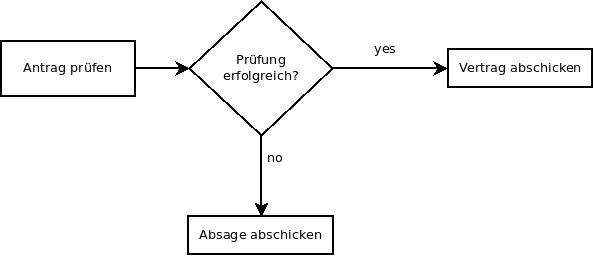
\includegraphics[width=0.7\textwidth]{Figures/sampleW}
	\caption{einfaches Beispiel eines Prozessschemas}
Ein einfaches Beispiel für das Schema eines Prozesses mit einem Start und zwei finalen Aktivitäten.In Abhängigkeit davon, welcher Wert für x berechnet wird, wird der Prozess entweder sofort abgebrochen, oder es werden weitere Aktivitäten ausgeführt.
	\label{fig2}
\end{figure}

Ein Prozessschema kann mehrere Instanzen besitzen, die mit \textbf{W$_i^k$} gekennzeichnet werden.
Eine Prozessinstanz $W_i^k$ ist eine Menge von Instanzen $T_i^k$ der zugehörigen Aktivitäten. Dabei ist $|T_i| \subseteq |T|$ eine Teilmenge aller möglichen Aktivitäten des zugehörigen Schemas, da einzelne Aktivitäten unter Umständen aufgrund der Abhängigkeiten nicht ausgeführt werden müssen.


%-----------------------------------
%	ACTIVITIES TASKS
%-----------------------------------
\subsection{Aktivitäten}
\label{sec:activities}
Eine Aktivität ist ein atomares Event, dh. eine in sich abgeschlossene Aufgabe im Kontext eines Prozesses. Sie haben eine definierte Menge von potentiellen Rollen und Nutzern, die die Erlaubnis besitzen, diese Aufgabe auszuführen. Sobald sie einem Nutzer zugewiesen wurde, kann kein weiterer Nutzer mehr die Aufgabe annehmen. Das bedeutet, dass jede Aktivität einen eindeutigen Nutzer und eine eindeutige Rolle hat, welcher sie ausgeführt hat.

Des weiteren besitzen die Aktivitäten einen eindeutigen Zeitstempel $\tau$, zu dessen Zeitpunkt sie ausgeführt wurden. Diese Zeitstempel bestimmen eine Ordnung $<T, \leq>$. Es gilt nämlich $t_1 < t_2 $, wenn $t_1$ vor $t_2$ ausgeführt wurde, dh. timestamp($t_1$) $<$ timestamp($t_2$).

Aktivitäten besitzen 7 verschiedene Zustände: \textit{new, scheduled, assigned, active, suspended, completed, aborted}. Die Aktivitäten werden durch \textbf{Events} von einem Zustand in den nächsten geführt. Die Übergänge können sehr fein gegliedert sein oder sich nur auf elementare \textit{Events} beschränken. In dieser Arbeit wird von 12 \textit{Event}-Typen ausgegangen: \textit{schedule, assign, reassign, start, complete, resume, suspend, autoskip, manualskip, withdraw, ate\_abort, pi\_abort}.

\begin{figure}[ht]
	\centering
  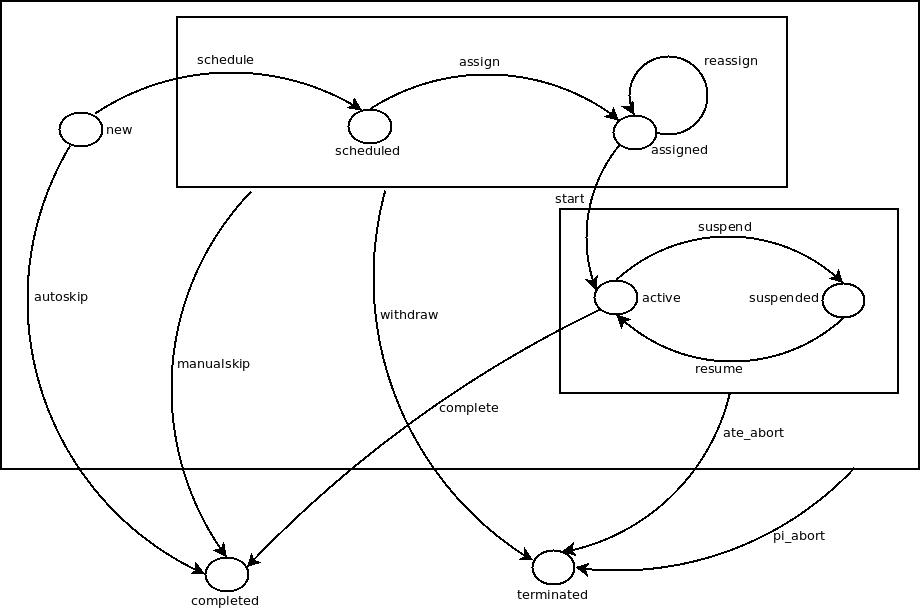
\includegraphics[width=0.9\textwidth]{Figures/Taskevents}
	\caption{Aktivitäten und Events}
Eine Aktivität und ihre möglichen Zustände. Der Startzustand ist \textit{new}. Die neue Aktivität kann entweder sofort verworfen werden oder wird einem Nutzer zugewiesen und gestartet. Es gibt die Möglichkeit, die Aufgabe einem anderen Nutzer zuzuweisen oder zu pausieren und wieder zu starten. Aus jedem Zustand heraus kann die Aktivität abgebrochen werden.
	\label{fig2}
\end{figure}
 

%-----------------------------------
%	ROLLENMODELL
%-----------------------------------
\subsection{Rollenmodell und Authorisierung}
Sei \textbf{T} = $\{t_1,t_2,...t_m\}$, $m\in\mathbb{N}$ eine Menge von Tasks, \textbf{R} = $\{r_1,r_2,...t_n\}$, $n\in\mathbb{N}$ eine Menge von Rollen, und \textbf{U} = $\{u_1,u_2,...u_l\}$,$l\in\mathbb{N}$ eine Menge von Usern.

\begin{figure}[ht]
	\centering
  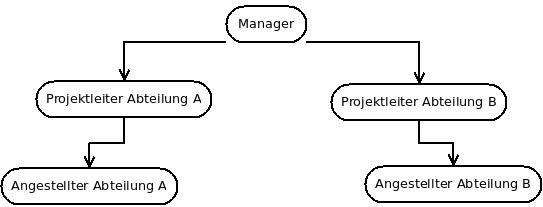
\includegraphics[width=0.9\textwidth]{Figures/Rollenmodell}
	\caption{Beispiel Rollenmodell}
	\label{fig:examplerolemodel}
\end{figure}

Eine \textbf{Authorisierung} ist eine Menge von potentiellen Nutzer und Rollen, denen es erlaubt ist, einen Task auszuführen. Eine Authorisierung besteht aus den Tupeln $$\textbf{TR} = (T\times R)$$ und $$\textbf{UR} = (U\times R)$$, welche eine n:m-Beziehung zwischen Tasks und Rollen, bzw zwischen Usern und Rollen kennzeichnen. Das bedeutet, dass User mit Rollen in der User-Rollen Beziehung assoziiert werden und Tasks mit Rollen in der Tast-Rollen Beziehung assoziiert werden.\\
Sei nun $$\textbf{R(t)} = \{r_m \in R: \exists(t_k, r_m) \in TR(t)\}$$
$$\textbf{U(t)} = \{u_n \in U: \exists(u_n, r_m) \in UR, r_m \in R(t)\}$$
Mit anderen Worten ist R(t) die Menge aller Rollen, die authorisiert sind, einen Task auszuführen und U(t) die Menge alles User, die authorisiert sind, einem Task zugeteilt zu werden.\\
Eine \textbf{Zuweisung} ist die konkrete Ausführung eines Tasks durch einen User.

Ein \textbf{hierarchisches Rollenmodell} ist eine geordnete Menge von Beziehungen zwischen Rollen $<R, \leq>$. Wenn $r_1, r_2 \in R$ und $r_1 < r_2$, dann dominiert die Rolle $r_2$ die Rolle $r_1$ in Bezug auf die organisatorische Rollenhierarchie. In Abb. \ref{fig:examplerolemodel} dominiert die Rolle "Projektleiter" die Rolle "Angestellter", das bedeutet, dass der "Projektleiter" alle Tasks ausführen darf, die der Rolle "Angestellter" zugeordnet wurde.
Die Rolle und all ihre Elternrollen bis zur Wurzel können einem Task zugewiesen werden.

\cite{wolter_modeling_of_TBAC_in_BPMN}

%-----------------------------------
%	ZEITMODELL
%-----------------------------------
\subsection{Zeitmodell}
Das Zeitmodell ist ein Tupel T = ($\Tau;\leq$).\\
$\Tau$ ist eine Menge von \textit{Zeitpunkten} $\tau$ und $\leq$ eine total Ordnung auf $\Tau$.
Ein \textit{Zeitinterval}$[\tau_a, \tau_b]$ ist eine Menge von Zeitpunkten $\tau \in \Tau$ mit $\tau_a \leq \tau \leq \tau_b$.
Ein Zeitinterval $\tau' = [\tau_a, \tau_b]$ wird als leer bezeichnet, falss $\tau_b \leq \tau_a$. \cite{warner_inter_instance}

\textbf{TS} wird als die Menge aller Zeitpunkt-Variablen und Konstanten wie 30.07.1999, 14:55 definiert und \textbf{TP} bezeichnet die Menge aller Zeitspannen wie 3 Tage 5 Stunden, 5 Monate.\\
Es gilt: $$TP - TP = TS$$ und $$TP + TS = TP$$ Die Differenz zwischen zwei Zeitpunkten ist eine Zeitspanne ( 30.07.1999 - 25.7.1999 = 5D ) und die Summe von einem Zeitpunkt und einer Zeitspanne ist wieder ein Zeitpunkt ( 25.07.1999 + 5D = 25.07.1999 ).




%-----------------------------------
%	Event Logs
%-----------------------------------
\subsection{Event Logs}

EventLogs sind Abbildungen von Prozessen $W_i$ auf eine Teilmenge $E \subseteq W_i$. Ein EventLog kann durchaus unvollständig sein bzw Fehler beinhalten. Jedoch wird in dieser Arbeit von einer \textit{Closed World} ausgegangen, was bedeutet, dass eine Aktivität, die nicht geloggt wurde, auch nicht stattgefunden hat.


\begin{figure}[h!]
	\centering
  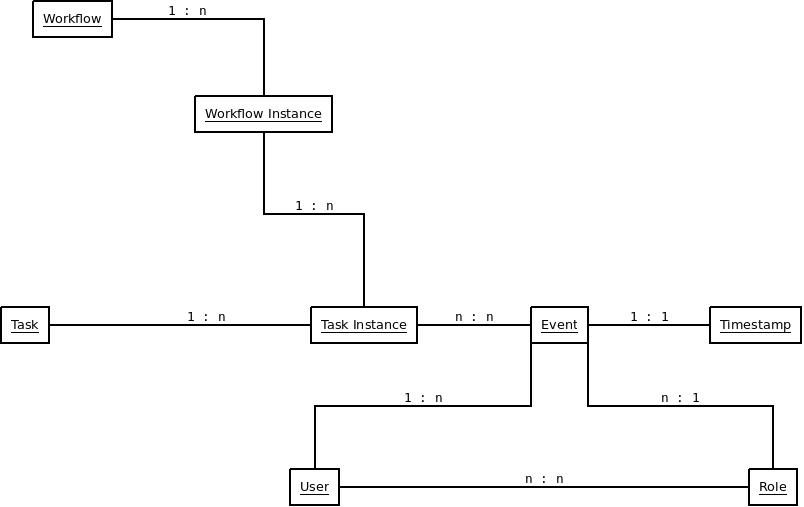
\includegraphics[width=0.9\textwidth]{Figures/WorkflowOntology}
	\caption{Ontologie eines Prozesses // TODO nochmal Beziehungen überdenken}
	\label{fig:ontology}
\end{figure}

// TODO Darstellung der additional Data, es ein bisschen verändern, damit man sieht, dass eine task von jedem element genau 1 hat

EventLogs repräsentieren die Instanzen eines Prozesses durch Auflistung der einzelnen Aktivitäten. In Tabelle \ref{tab:examplelog} wird ein exemplarischer Log dargestellt. Die \textit{caseID} kennzeichnet die Instanz des Prozesses, da ein Prozessschema mehrere Instanzen besitzen kann. Zu einer Prozessinstanz können mehrere Aktivitäten (hier \textbf{Task}) gehören, die jedoch einen eindeutigen Zeitstempel, Eventtypen, Nutzer und dessen Rolle haben. Zudem kann eine Aktivität beliebig viele zusätzliche Informationen besitzen, die in dieser Tabelle nur angedeutet werden.

\begin{table}[h!]
\footnotesize
  \centering
  \begin{tabular}{|c|c|c|c|c|c|c|}
  \hline
  caseID & Task & User & Role & Timestamp & EventType & DataAttributes\\
  \hline
  0 & Approach check &'Mark' &'Admin' &1999-12-13T12:22:15 & start&(amount, 3000)\\
  0 & Pay check & 'Theo' &'Azubi' &1999-12-13T12:22:16 & start&(amount, 3000Euro)\\
  1 & Approach check &'Lucy' & 'Azubi' &1999-12-13T12:22:17 &start&(customer, Max Muster)\\
  1 & Pay check &'Mark' & 'Admin' &1999-12-13T12:22:18 & abort&()\\
  0 & Revoke check & 'Theo' & 'Clerk' & 1999-12-13T12:22:19 & start&()\\
  \hline
  \end{tabular}
\\
Das ist nur ein Auszug und kein vollständiger Log. Es können auch weitere Daten vorhanden sein, die hier nicht dargestellt werden.
  \caption{Beispiel Log Einträge. }
  \label{tab:examplelog}
\end{table}



%-----------------------------------
%	Security policy
%-----------------------------------
\subsection{Schutzziele}

Um bestimmen zu können, welche Regeln und Einschränkungen für den Ablauf eines Prozesses notwendig sein könnten, muss zuletzt noch auf die Schutzziele von Unternehmen (besseres Wort) eingegangen werden.

Müller et al. \cite{mueller_accorsi} sammeln unter anderem\footnote{Ein weiteres Schutzziel ist "Data Integrity" und "Nutzungskontrolle", welches für diese Arbeit nicht relevant ist.} folgende Punkte:\\

\textbf{(1) Autorisierung}\\
Welche Subjekte bzw Rollen dürfen auf welche Ressourcen zugreifen? Da es in größeren Unternehmen komplex werden kann, wurde das Rollenmodell zur Vereinfachung entwickelt. \\
\textbf{(2) Nutzungskontrolle}\\
Regelt die Art der Nutzung. RWX, begrenzte Anzahl an Zugriffen, bzw Verpflichutung einer Löschoperation (weiteren, resultierenden Handlungen) nach Zugriff(Kontrollfluss)\\
\textbf{(3) Interessenskonflikt}\\
Unterbindung von unzulässiger Ausnutzung von insider-Wissen. Chinese Wall Modell.\\
\textbf{(4) Funktionstrennung}\\
Bestimmte Aufgaben dürfen nicht vom selben Subjekt, Rolle, Abteilung, ausgeführt werden. Unterbindung von kriminellen Handlungen und Betrug.\\
\textbf{(5) Aufgabenbindung}\\
Gegenteil von Funktionstrennung\\
\textbf{(6) Mehr-Augen-Kontrolle}\\
kritische Aktivität im Prozess darf nicht von einer einzelnen Person ausgeführt werden. Das wäre bei mir Cardinality Constraints, wenn eine Aktivität aus mehreren Tasks besteht.\\

// TODO: was kann man noch hinzufügen?



\section{Herleitung der Einschränkungen}


%-----------------------------------
%	Definition Constraints
%-----------------------------------

\subsection{Ein praktisches Beispiel mit vielen Einschränkungen}
\label{sec:exampleconstraints}

In diesem Kapitel werden verschiedene Arten von Einschränlungen und Regeln betrachtet.
Constraints sind Regeln bzw Einschränkungen, die aus dem Verlauf von vorhergehenden Tasks resultieren. Einschränkungen und Regeln werden hier synonym verwendet.
Einschränkungen haben den Zweck Betrug, aber auch menschliches Versagen zu verhindern.
Um sich ein besseres Bild von Einschränkungen zu machen, betrachten wir vor der eigentlichen Analyse ein Beispiel, welches im Verlauf der Arbeit auf die Einhaltung der Regeln untersucht wird.
Das folgende Beispiel wurde in leicht veränderter Form \cite{wolter_modeling_of_TBAC_in_BPMN} entnommen. // TODO stimmt das überhaupt?

Der Prozess in Abbildung \ref{fig:Workflow} stellt die Bearbeitungsschritte eines Kreditantrages in einer Bank dar. In (T1 - Antrag empfangen) müssen zuerst alle erforderlichen Daten des Kunden aufgenommen werden. Daraufhin muss der Antrag geprüft werden, wie zum Beispiel die Kreditwürdigkeit des Kunden (T2 - Antrag prüfen). Sollte der gewünschte Betrag des Kredites 100000 Euro übersteigen, muss der Antrag zur Sicherheit von einer weiteren Person geprüft werden (T3 - Antrag prüfen). Nun muss entweder ein Vertrag vorbereitet werden (T4) oder, falls die Prüfung negativ verlaufen ist, ein Schreiben vorbereitet werden, welches dan Antrag ablehnt (T5). Unabhängig von dem Ergebnis wird der Kunde zuletzt noch einmal kontaktiert (6).
\begin{figure}[ht]
	\centering
  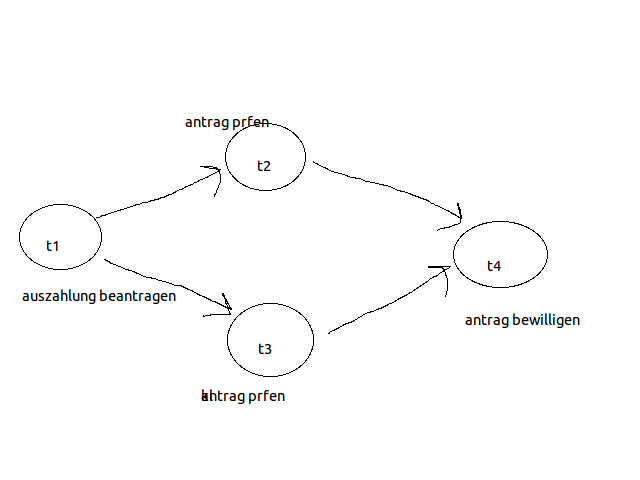
\includegraphics[width=0.9\textwidth]{Figures/Workflow}
	\caption{Bearbeitung eines Kreditantrags in der Bank}
	\label{fig:Workflow}
\end{figure}
\\
Um einen sicheren und reibungslosen Ablauf zu gewährleisten, werden folgende Anforderungen gestellt:

\begin{enumerate}
\item (Der Kontakt mit Kunden) T1 und T6 muss vom Kundenberater erledigt werden
\item Um den Kunden nicht zu lange warten zu lassen, sollte der Kunde spätestens 3 Tage nach erstem Kontakt über das Ergebnis informiert werden (timestamp(T6) $<$ timestamp(T1) + 3D)
\item Um zu verhindern, dass Fehler durch Überlastung passieren, darf jeder Mitarbeiter am Tag höchstens 100 Tasks bearbeiten.
\item Den Antrag annehmen (T1) und den Antrag prüfen(T2, T3) sollten von verschiedenen Personen erledigt werden (4 Augen Prinzip).
\item Ferner sollten auch die zwei Prüfungen von verschiedenen Mitarbeitern vollzogen werden. T3 muss durch den Bank Manager erfolgen.
\item Wenn ein Mitarbeiter 5x einem Task zugewiesen wird und ihn dann abbricht, darf er nicht mehr an dem Task arbeiten.
\item Es dürfen keine Anträge von Verwandten geprüft werden.
\item Es dürfen auch höchstens 3 mal Mitarbeiter an den Anträgen des jeweils anderen Verwandten arbeiten.
\item Ein Mitarbeiter darf bei dem selben Kunden höchstens Kredite bis 100000 Euro prüfen.
\item Es dürfen hochstens 3 mal die selben Personen an T2 und T3 arbeiten
\end{enumerate}


%
% Arten von Constraints
%
\subsection{Arten von Constraints - Herleitung}
\label{sec:ArtenConstraints}

Generell kann man verschiedene Arten von Regeln erkennen.\\

\begin{figure}[ht]
	\centering
  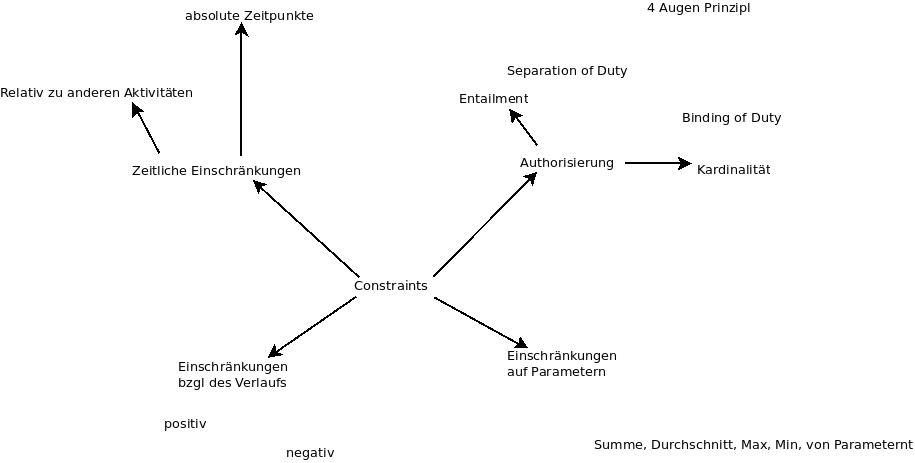
\includegraphics[width=0.9\textwidth]{Figures/Constraints}
	\caption{Typen von Einschränkungen und regeln}
	\label{fig:constraints}
\end{figure}

\textbf{Sich gegenseitig ausschließende Tasks (Conflicting Tasks)}
TODO: kommt das zur Constraint Sammlung?
In manchen Fällen kann man Tasks nicht verschiedenen Rollen zuweisen  ohne die exisitierenden Rollen derart zu segmentieren, dass die schwer zu verwalten sind in Bezug auf das organsiatorische Modell. Außerdem können Rollenhierarchien dazu verwendet werden, in zwei verschiedenen Rollen zu agieren, die eigentlich getrennt waren. ZB könnte ein Manager als ein Clerk und gleichzeitig als sein eigenener Supervisor handeln.\\
Deswegen definieren wir \textbf{TC} $\subset$ T als eine Menge von \textbf{kollidierenden Tasks}. TC beinhaltet Tasks, deren Allokation von der Allokation von vorhergehend ausgeführten Tasks aus TC abhängt. Diese Abhängigkeit wird als Abhängigkeit zwischen Tasks aus TC beschrieben. $t_c\in TC$ gilt als entailed Task von $t_m\in TC$, wenn die Allokation von $t_n$ von der Allokation von $t_m$ eingeschränkt wird, mit $t_m<t_n$.
\cite{wolter_modeling_of_TBAC_in_BPMN}\\

\textbf{Zeitliche Beschränkungen}\\
--absolute Einschränkungen\\
Das sind Einschränkungen, die sich auf einen absoluten Zeitpunkt beziehen, wie zum Beispiel dass besondere Kredite nicht mehr vergeben werden dürfen, nachdem das Angebot erloschen ist. Sollte nach dem festgelegten Datum trotzdem dieser Kredit vergeben werden, stellt das einen Regelbruch dar.
--relative Einschränkungen\\
Relative Einschränkungen beziehen sich auf vorher erfüllte Aufgaben und schränken die weiteren für einen bestimmten Zeitraum ein.\\

\textbf{Einschränkungen auf Parametern}\\
Einschränkungen, die mit der Akkumulation von Aktivitäten arbeiten, geben oft eine Grenze für einen Parameter in einem bestimmten Zeitraum vor. Diese Art der Einschränkungen ist oft mit zeitlichen Einschränkungen verbunden.\\

\textbf{Entailment Constraint}
c=(TC, $n_u$,$m_{th}$) mit $n_u$ als minimale Anzahl an verschiedenen Usern, die einem Task zugewiesen werden müssen. Wenn $t_{ki}$ eine Instanz des Tasks $t_k$ ist, dann ist $m_th$ der Grenzwert von der Summe der Task Instanzen, denen ein User zugewiesen sein darf.
\cite{wolter_modeling_of_TBAC_in_BPMN}
\textbf{Separation of Duty}\\
...\\
\textbf{Binding of Duty Constraints}\\
...\\
\textbf{Cardinality Constraints}\\
..\\
\textbf{Workflow Soundness}\\
Das sind Regeln, die allgemein den korrekten Ablauf eines Prozesses sicherstellen sollen. Diese Regeln beziehen sich im Allgemeinen nicht darauf, welcher Nutzer eine Aktivität ausgeführt hat (keine Authorisierungs-Einschränkungen) sondern betrachten die Tatsache, ob eine Aktivität zu einem korrekten Zeitpunkt oder in einem korrekten Zusammenhang ausgeführt wurde.

TODO Zum ein oder anderen Vielleicht Quellenangabe

\subsection{Gültigkeitsbereich von Constraints}
//TODO Welche der Einschränkungen gehört wohin
\textbf{Intra-Instanz}\\
Die meisten Ansätze beziehen sich auf Regeln, die in Bezug zu einer Prozessinstanz stehen. Hier gilt, dass die Prozessinstanz für alle Aktivitäten die selbe ist. Sollten zwei Aktivitäten zu verschiedenen Instanzen gehören, werden sie nicht gegeneinander betrachtet. Seien A und B zwei Aktivitäten, dann gilt A.caseID = B.caseID. 
\\
\textbf{Inter Instanz}\\
Wie bereits erkannt wurde, reicht es nicht aus, nur Einschränkungen innerhalb eines Prozesses zu definieren, da sich eine kriminelle Handlung auch über mehrere Instanzen bemerkbar machen kann. TODO Weitere Erklärung oder kleineres Beispiel. Die Einschränkung von oben wird hier aufgehoben, es gilt jedoch noch, dass die betrachteten Tasks zum selben Prozessschema gehören müssen, dh A.case = B.case
\\
\textbf{Inter-Prozess}\\
Die Regeln beziehen sich auf alle Aktivitäten, unabhängig davon, zu welcher Prozessinstanz oder welchem Prozessschema sie gehören. Diese Einschränkungen betrachten häufig die Akkumulation von verschiedenen Aktivitäten, ihre Anzahl bzw Operationen auf die Aggregation ihrer Parameter.

